\documentclass[dvipsnames,table,mathserif,aspectratio=169]{beamer} % Definição do tipo de arquivo

\usepackage[T1]{fontenc}     	 %---------------------------------%
\usepackage[utf8]{inputenc} 	 % Para língua portuguesa          %
\usepackage[brazil]{babel}    %---------------------------------%
\usepackage{times}
\usepackage[framesassubsections]{beamerprosper} % opiniõs: email, institution,
\usepackage{algorithmic}
\usepackage{graphicx,url}
\usepackage{enumerate}
\usepackage{amsmath,amsfonts,amsthm,bbm,amssymb}
\usepackage{epsfig}
\usepackage{booktabs}
\usepackage{caption}
\usepackage{scalefnt}
\usepackage[caption=true,font=footnotesize]{subfig}
\usepackage{multimedia}

\usepackage[round]{natbib}
\bibpunct{(}{)}{;}{a}{}{;}

%\newcommand{\newblock}{}
\usetheme{CambridgeUS}
\usecolortheme{whale}
%\renewcommand{\sfdefault}{times}
\setbeamercolor{alerted text}{fg=blue!80!black}
\setbeamercolor{frametitle}{fg=blue!80!black}
\setbeamercolor{block title}{bg=blue!90!black,fg=white}
\beamertemplatetransparentcovereddynamicmedium

\title[]{\textbf{Uma Plataforma Web para Gerenciamento de Dados e Geração de Boletins Meteorológicos do LabInstru}\\ \small{Trabalho de Conclusão de Curso II}}

\author[Pedro Ribeiro]{\textbf{Pedro Augusto Franco Ribeiro}\\\email{pafr.eng@uea.edu.br}\\\ \ \newline \small{Orientadoras: Elloá B. Guedes, Maria Betânia Leal de Oliveira}\\}
\institute[NUCOMP, EST, UEA]
{
  Núcleo de Computação\\
  Escola Superior de Tecnologia\\
  Universidade do Estado do Amazonas\\
  Manaus -- Amazonas -- Brasil
}

\begin{document}
\selectlanguage{brazil}

\maketitle % Título da apresenta��o

\AtBeginSection[]
{
	\begin{frame}{Outline}
		\tableofcontents[currentsection]
	\end{frame}
}

\section{Introdução}
\begin{frame}{Introdução}
\begin{itemize}
\item Tecnologias computacionais auxiliam no processamento de dados
\ \ \newline
\item \alert{Meteorologia} é a ciência responsável pelo estudo do clima e tempo
\begin{itemize}
	\item Demanda por armazenamento, processamento e gerenciamento dos dados meteorológicos
	\item Necessidade  de confiabilidade e rapidez no processamento das informações
\end{itemize}
\end{itemize}
\end{frame}

\begin{frame}{Introdução}
\begin{itemize}
\item LabInstru: Laboratório de Instrumentação Meteorológica
\begin{itemize}
	\item Localizado na Escola Superior de Tecnologia (EST)
	\item Sala C29
	\item Universidade do Estado do Amazonas (UEA)
\end{itemize}
\ \ \newline
\item Administra a \alert{Estação Meteorológica Automática} da EST
\begin{itemize}
	\item Em funcionamento desde 2010
	\item Coleta de diversas variáveis meteorológicas
	\item Processamento e disponibilização dos dados
	\item Geração de boletins meteorológicos
\end{itemize}
\end{itemize}
\end{frame}

\begin{frame}{Introdução}
\begin{itemize}
\item Exemplo de arquivo-texto oriundo da estação meteorológica:
\end{itemize}

\begin{figure}
\centering
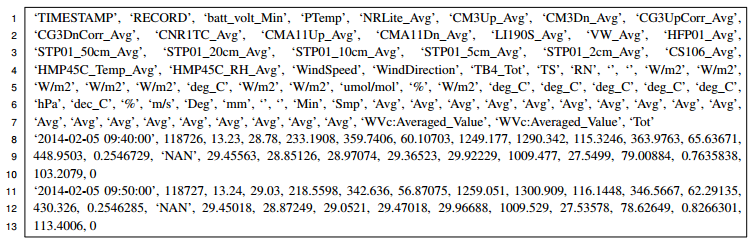
\includegraphics[width=0.9\linewidth]{./img/dat}
%\caption{Exemplo de um trecho dos dados encontrados no arquivo produzido pela estação meteorológica.} \label{fig:exemploBaixa1}
\end{figure}

\end{frame}

\begin{frame}{Introdução}

\begin{block}{Problemas Identificados}
	\begin{itemize}
		\item Processamento de dados feito de maneira manual
		\item Processo demorado e exaustivo
		\item Resultados sujeitos a erros e imprecisões
		\item Requer mão de obra especializada
	\end{itemize}
\end{block}
\ \ \newline

\end{frame}

\begin{frame}{Introdução}

\begin{block}{Objetivo Geral}
	\begin{itemize}
		\item Projetar e implementar uma plataforma web para armazenamento, gerenciamento e disponibilização de dados de uma estação meteorológica automática
	\end{itemize}
\end{block}
\ \ \newline

\begin{block}{Objetivos Específicos}
	\begin{itemize}
		\item Identificar e documentar as funcionalidades a serem desenvolvidas
		\item Elaborar protótipos de interface para validar as funcionalidades
		\item Levantamento das tecnologias utilizadas para o desenvolvimento da aplicação
		\item Projetar e implementar a plataforma web
		\item Implantar a plataforma web no LabInstru
	\end{itemize}
\end{block}
\ \ \newline

\end{frame}

\begin{frame}{Introdução}
\begin{block}{Metodologia}
	\begin{enumerate}
	\item Identificação de um processo de desenvolvimento
	\item Estudos dos arquivos gerados pela estação meteorológica
	\item Elicitação de requisitos
	\item Construção protótipos de interface gráfica
	\item Definição de uma agenda de implementação
	\item Identificação de tecnologias
	\item Implementação
	\item Escrita e defesa do TCC1
	\item Implantação
	\item Escrita e defesa do TCC2
\end{enumerate}
\end{block}


\end{frame}


\section{Solução Proposta}
\begin{frame}{Solução Proposta: Processo de Desenvolvimento}
\begin{itemize}
	\item Processo de Desenvolvimento Adotado: \alert{Processo Unificado Ágil}
	\begin{itemize}
		\item Fases e disciplinas
		\item Concepção, elaboração, construção e transição
	\end{itemize}
	\ \ \newline
	\item Aplicação a ser desenvolvida não é considerada de grande porte
	\ \ \newline
	\item Papéis:
	\begin{itemize}
		\item Desenvolvedor e testador: Pedro Augusto
		\item Cliente: Profa. Maria Betânia
		\item Solicitante do software e Gerente do Projeto: Profa. Elloá
	\end{itemize}
\end{itemize}
\end{frame}

\begin{frame}{Solução Proposta}
\begin{block}{Elicitação de Requisitos}
\begin{itemize}
	\item Identificação dos requisitos funcionais e não funcionais
	\item Identificação de quatro módulos principais:
	\begin{enumerate}
		\item Módulo Gerencia Conta de Usuário
		\item Módulo Usuário
		\item Módulo Consulta Medições
		\item Módulo Gerencia Medições
	\end{enumerate}
\end{itemize}
\end{block}

\end{frame}

\begin{frame}{Solução Proposta: Diagramas de Caso de Uso}
\begin{figure}[h!]
\centering
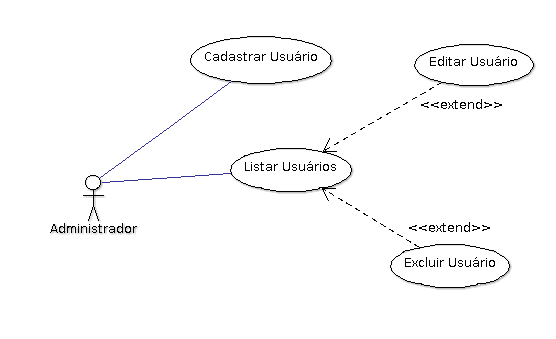
\includegraphics[width=0.8\linewidth]{./img/uc001}
\end{figure}
\end{frame}

\begin{frame}{Solução Proposta: Diagramas de Caso de Uso}
\begin{figure}[h!]
\centering
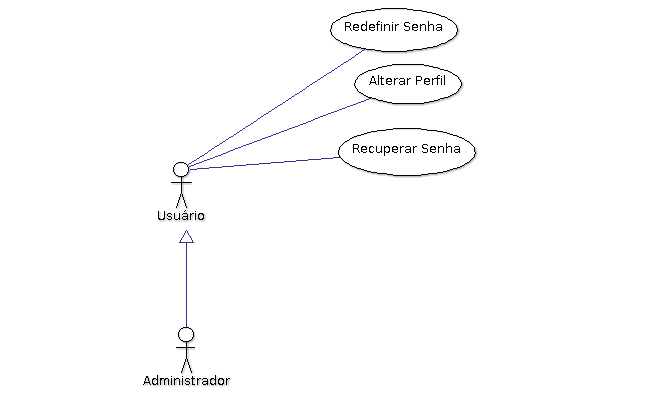
\includegraphics[width=0.7\linewidth]{./img/uc002}
\end{figure}
\end{frame}

\begin{frame}{Solução Proposta: Diagramas de Caso de Uso}
\begin{figure}[h!]
\centering
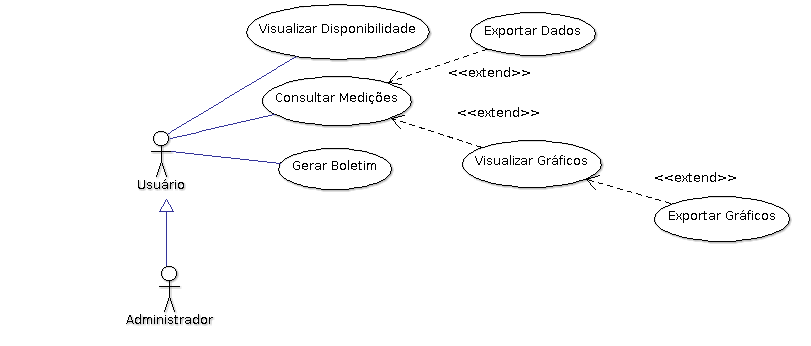
\includegraphics[width=1\linewidth]{./img/uc003}
\end{figure}
\end{frame}

\begin{frame}{Solução Proposta: Diagramas de Caso de Uso}
\begin{figure}[h!]
\centering
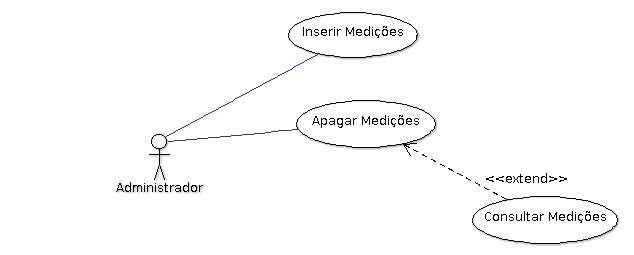
\includegraphics[width=1\linewidth]{./img/uc004}
\end{figure}
\end{frame}


\begin{frame}{Solução Proposta}
\begin{block}{Elaboração de Modelos}
\begin{itemize}
	\item Identificação das principais abstrações efetuadas e da associação entre elas
	\item Modelo Conceitual
	\item Modelo Entidade-Relacionamento
\end{itemize}
\end{block}
\end{frame}

\begin{frame}{Solução Proposta: Modelo Conceitual}
	\begin{figure}[h!]
	\centering
	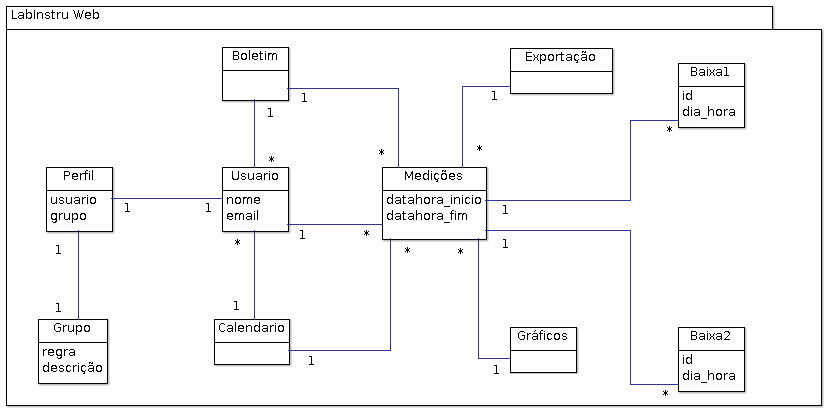
\includegraphics[width=0.8\linewidth]{./img/ModeloConceitual}
	\end{figure}
\end{frame}

\begin{frame}{Solução Proposta: Modelo Entidade-Relacionamento}
	\begin{figure}[h!]
	\centering
	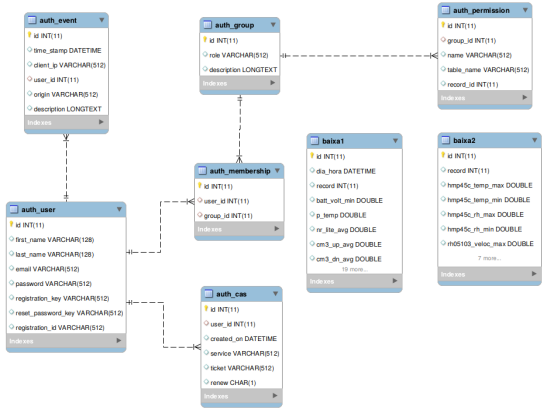
\includegraphics[width=0.6\linewidth]{./img/mer}
	\end{figure}
\end{frame}

\begin{frame}{Solução Proposta}
\begin{block}{Prototipação das Telas do Usuário}
\begin{itemize}
	\item Elaboração de protótipos da interface com o usuário
	\item Representação limitada da solução, mas capaz de explorar a sua conveniência
	\item Utilização do Balsamiq Mockups
\end{itemize}
\end{block}
\end{frame}

\begin{frame}{Solução Proposta: Prototipação}
\begin{figure}[h!]
\centering
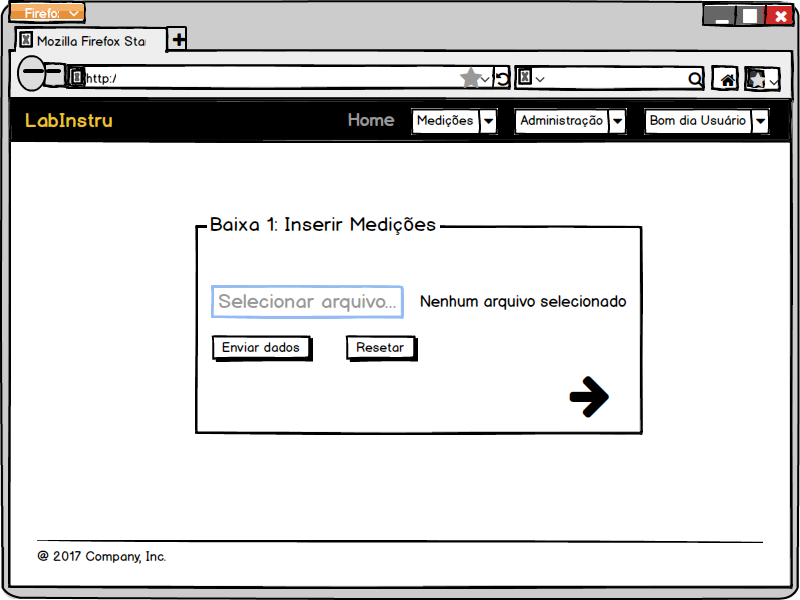
\includegraphics[width=0.6\linewidth]{./img/tela053}
\caption{Protótipo cadastra medições} \label{fig:uc001}
\end{figure}
\end{frame}

\begin{frame}{Solução Proposta: Prototipação}
\begin{figure}[h!]
\centering
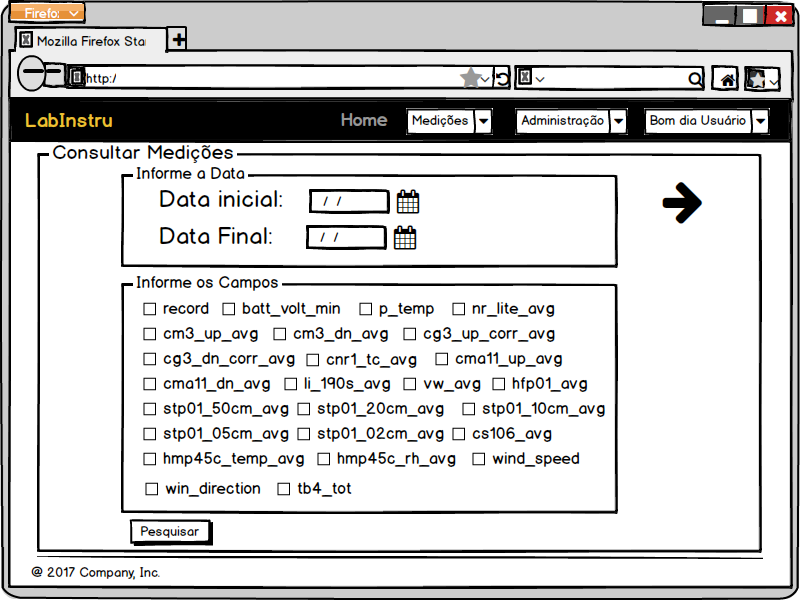
\includegraphics[width=0.6\linewidth]{./img/tela058}
\caption{Protótipo consulta medições} \label{fig:uc001}
\end{figure}
\end{frame}



\begin{frame}{Solução Proposta}
	\begin{block}{Implementação}
		\begin{itemize}
			\item \alert{LabInstru Web}: plataforma web proposta para atender às necessidades identificadas no LabInstru
			\ \ \newline
			\item \emph{Framework} utilizado: Web2py
				\begin{itemize}
					\item Programável e escrito em Python
					\item Utiliza o MVC como padrão de projeto
				\end{itemize}
			\ \ \newline
			\item Melhorias na interface com o usuário:
			\begin{itemize}
				\item \emph{Framework} Bootstrap
				\item Biblioteca JQuery
			\end{itemize}
			\ \ \newline
			\item Sistema gerenciador de Banco de Dados: MySQL
		\end{itemize}
	\end{block}
\end{frame}

\begin{frame}{Solução Proposta: Funcionalidades Implementadas}
\begin{figure}[h!]
\centering
\frame{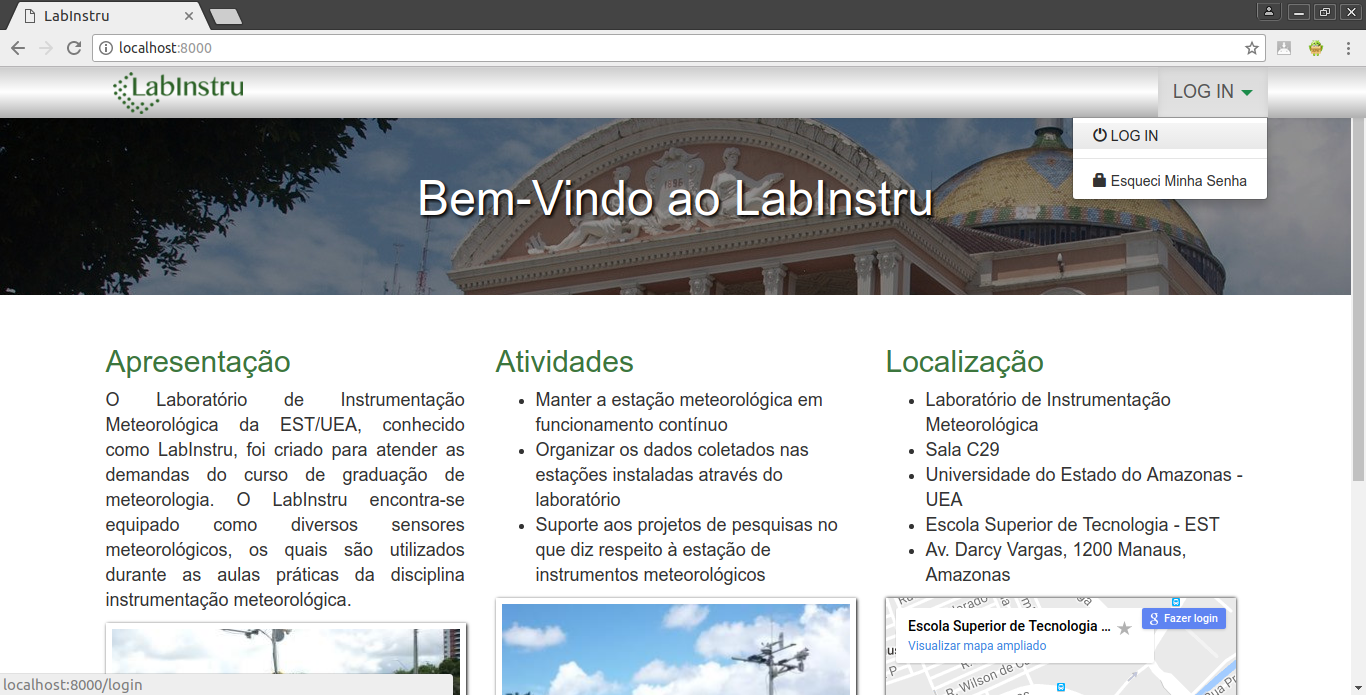
\includegraphics[width=0.7\linewidth]{./img/ap1}}
\caption{Página inicial da aplicação.}
\end{figure}
\end{frame}

\begin{frame}{Solução Proposta: Funcionalidades Implementadas}
\begin{figure}[h!]
\centering
\frame{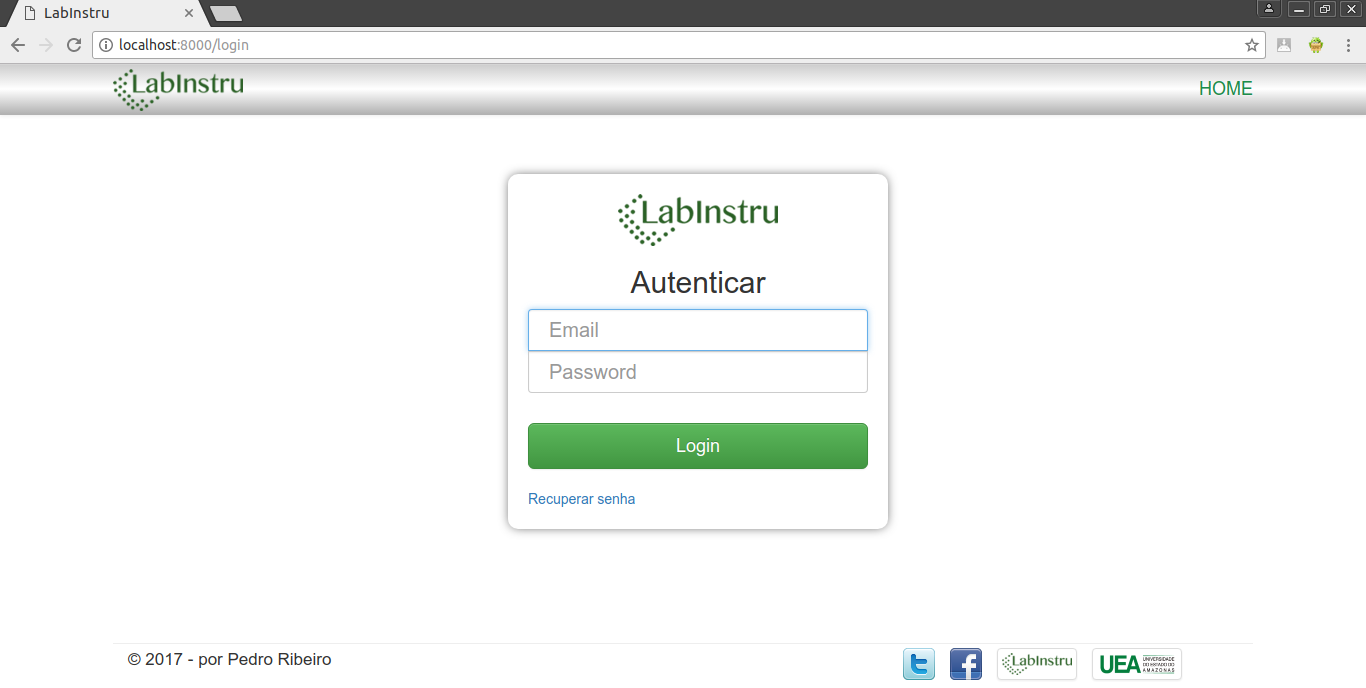
\includegraphics[width=0.7\linewidth]{./img/ap10}}
\caption{Autenticação de usuários.}
\end{figure}
\end{frame}

\begin{frame}{Solução Proposta: Funcionalidades Implementadas}
\begin{figure}[h!]
\centering
\frame{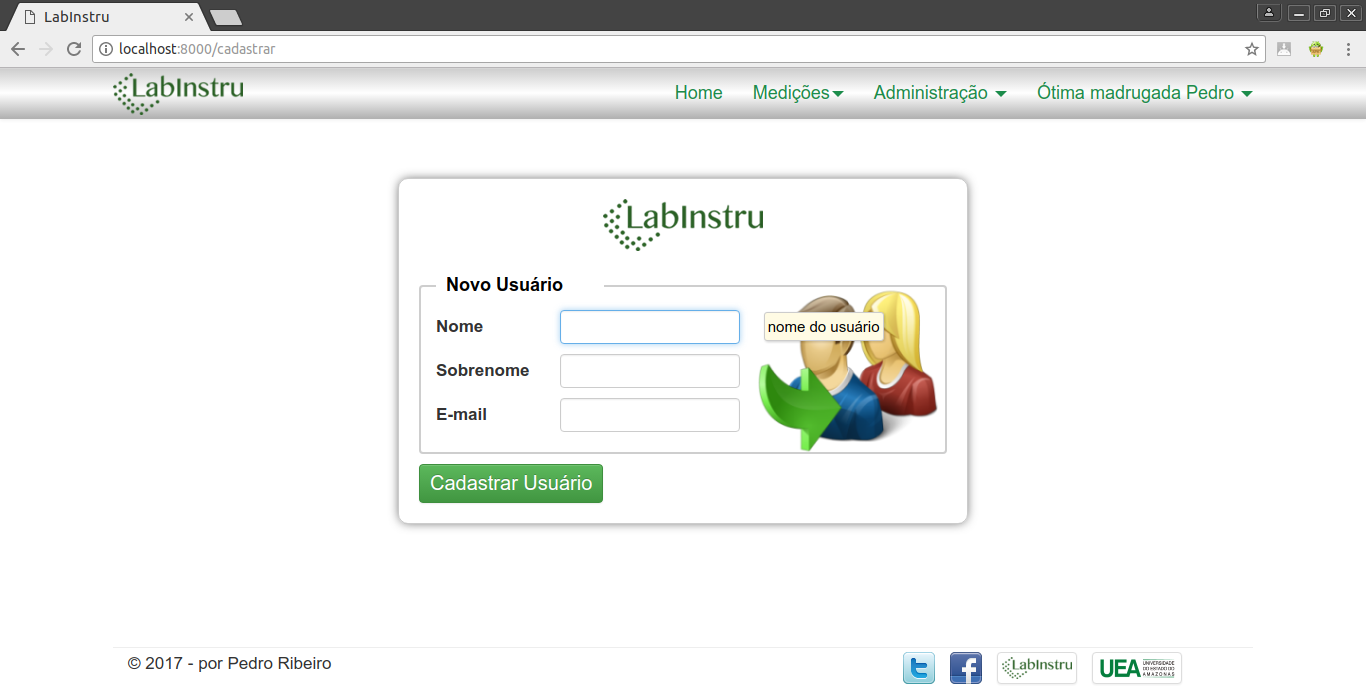
\includegraphics[width=0.7\linewidth]{./img/ap4}}
\caption{Cadastro de usuários.}
\end{figure}
\end{frame}

\begin{frame}{Solução Proposta: Funcionalidades Implementadas}
\begin{figure}[h!]
\centering
\frame{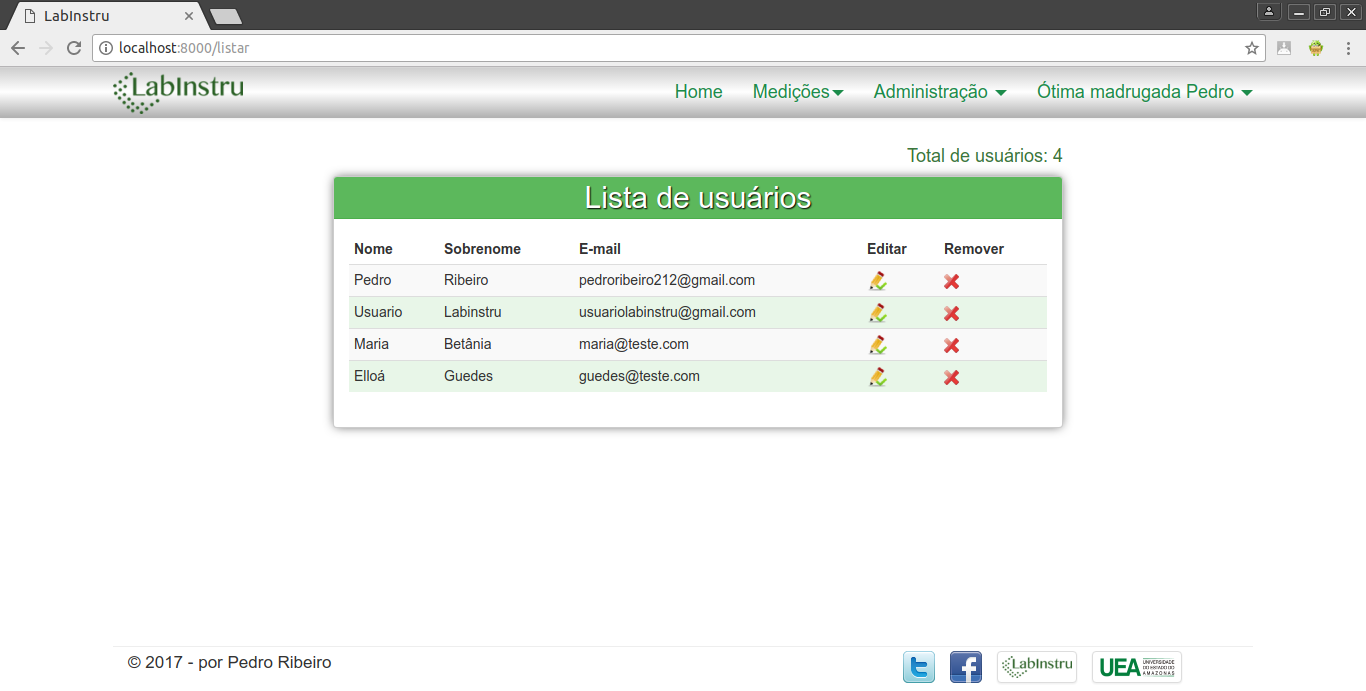
\includegraphics[width=0.7\linewidth]{./img/ap14}}
\caption{Listagem de usuários.}
\end{figure}
\end{frame}


\begin{frame}{Solução Proposta: Funcionalidades Implementadas}
\begin{figure}[h!]
\centering
\frame{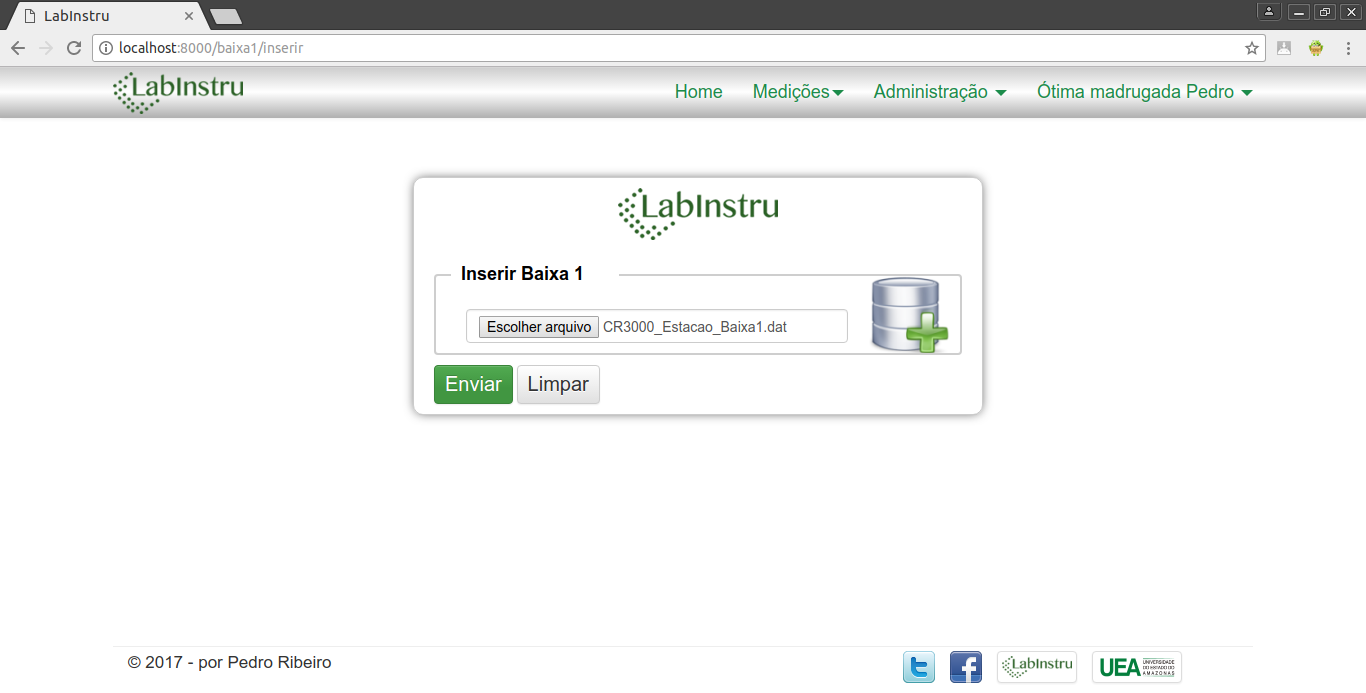
\includegraphics[width=0.7\linewidth]{./img/ap12}}
\caption{Cadastro de Medições.}
\end{figure}
\end{frame}

\begin{frame}{Solução Proposta: Funcionalidades Implementadas}
\begin{figure}[h!]
\centering
\frame{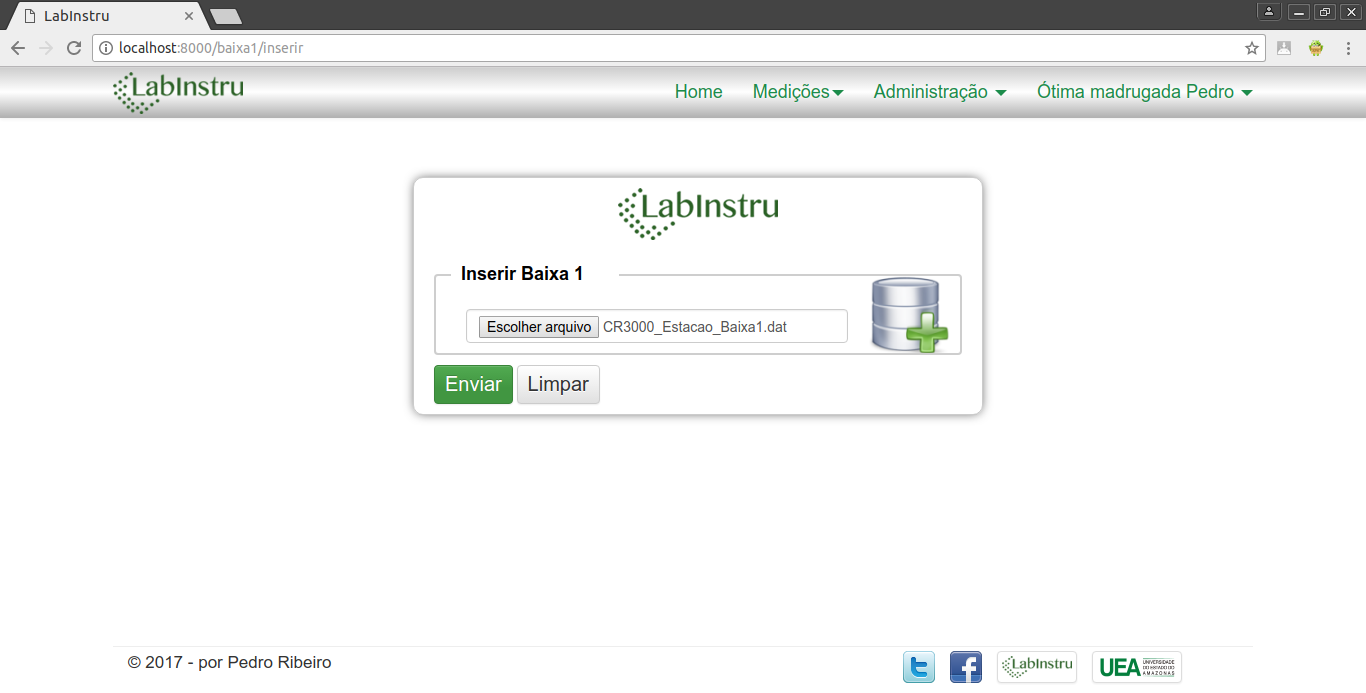
\includegraphics[width=0.7\linewidth]{./img/ap12}}
\caption{Cadastro de Medições.}
\end{figure}
\end{frame}

\begin{frame}{Solução Proposta: Funcionalidades Implementadas}
\begin{figure}[h!]
\centering
\frame{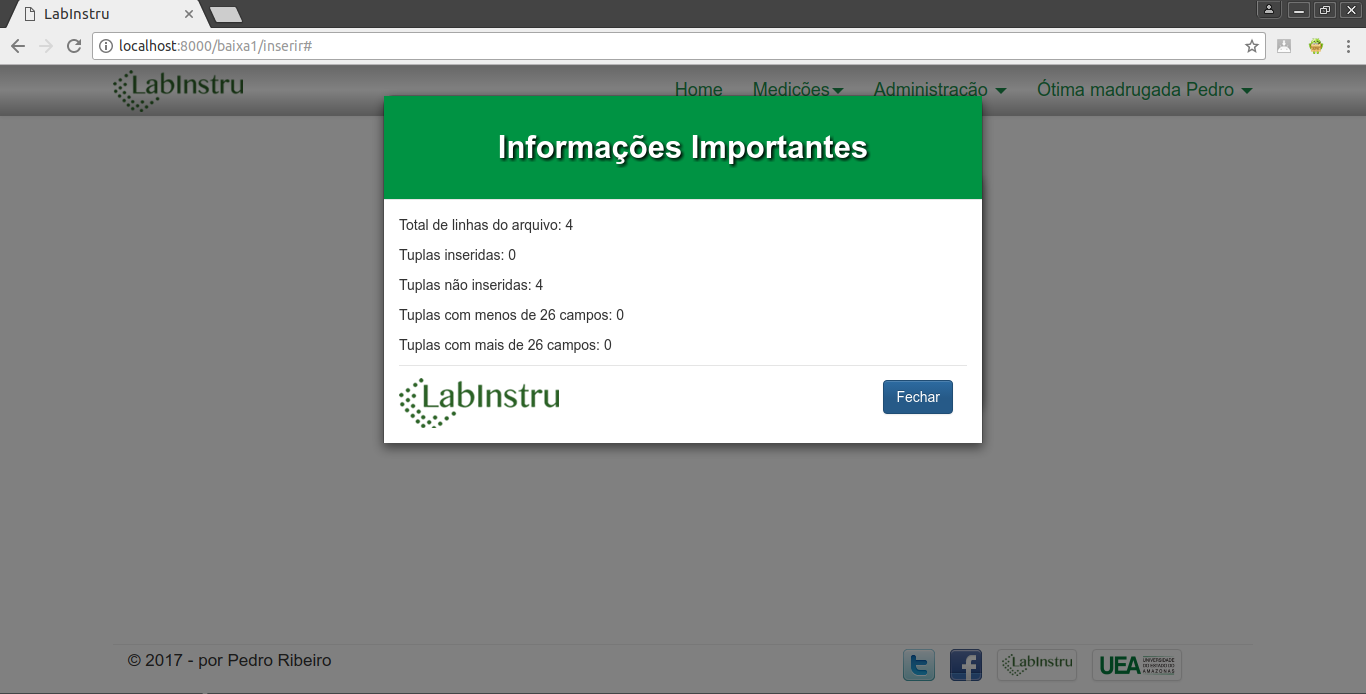
\includegraphics[width=0.7\linewidth]{./img/ap13}}
\caption{Log resultante do cadastro de Medições.}
\end{figure}
\end{frame}

\begin{frame}{Solução Proposta: Funcionalidades Implementadas}
\begin{figure}[h!]
\centering
\frame{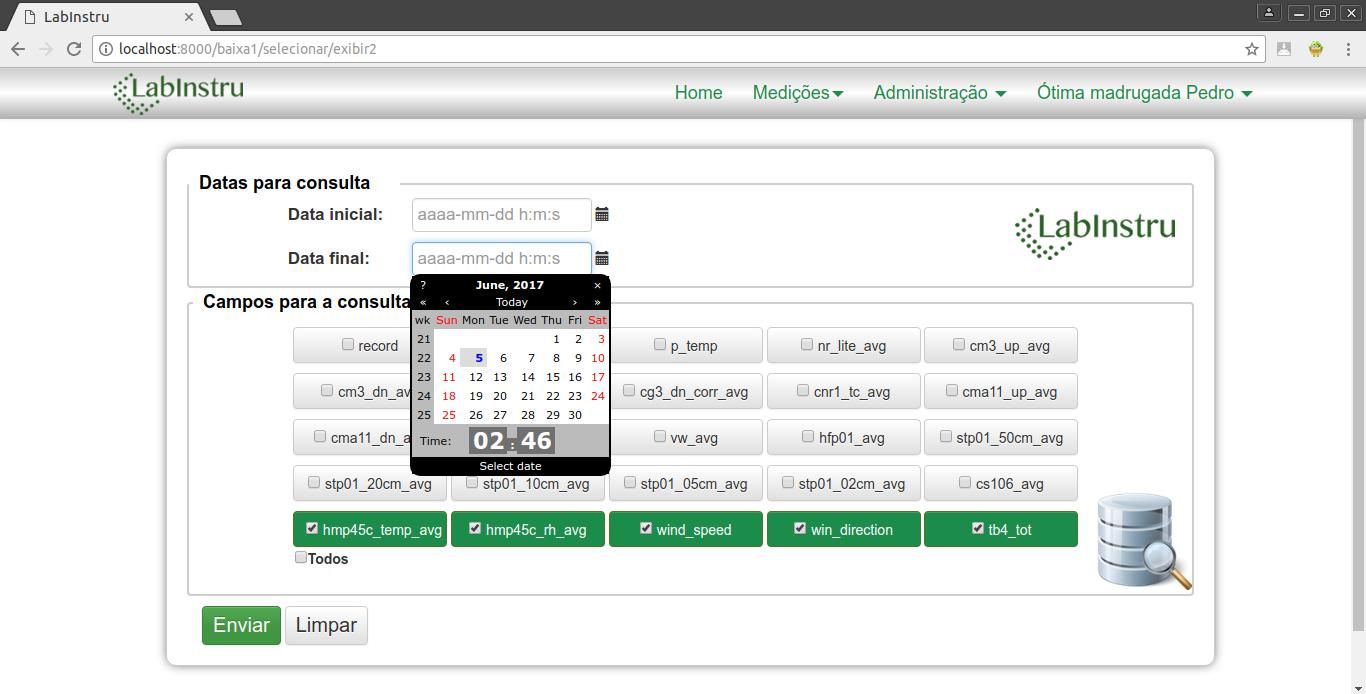
\includegraphics[width=0.7\linewidth]{./img/ap3}}
\caption{Consulta de medições.}
\end{figure}
\end{frame}

\begin{frame}{Solução Proposta: Funcionalidades Implementadas}
\begin{figure}[h!]
\centering
\frame{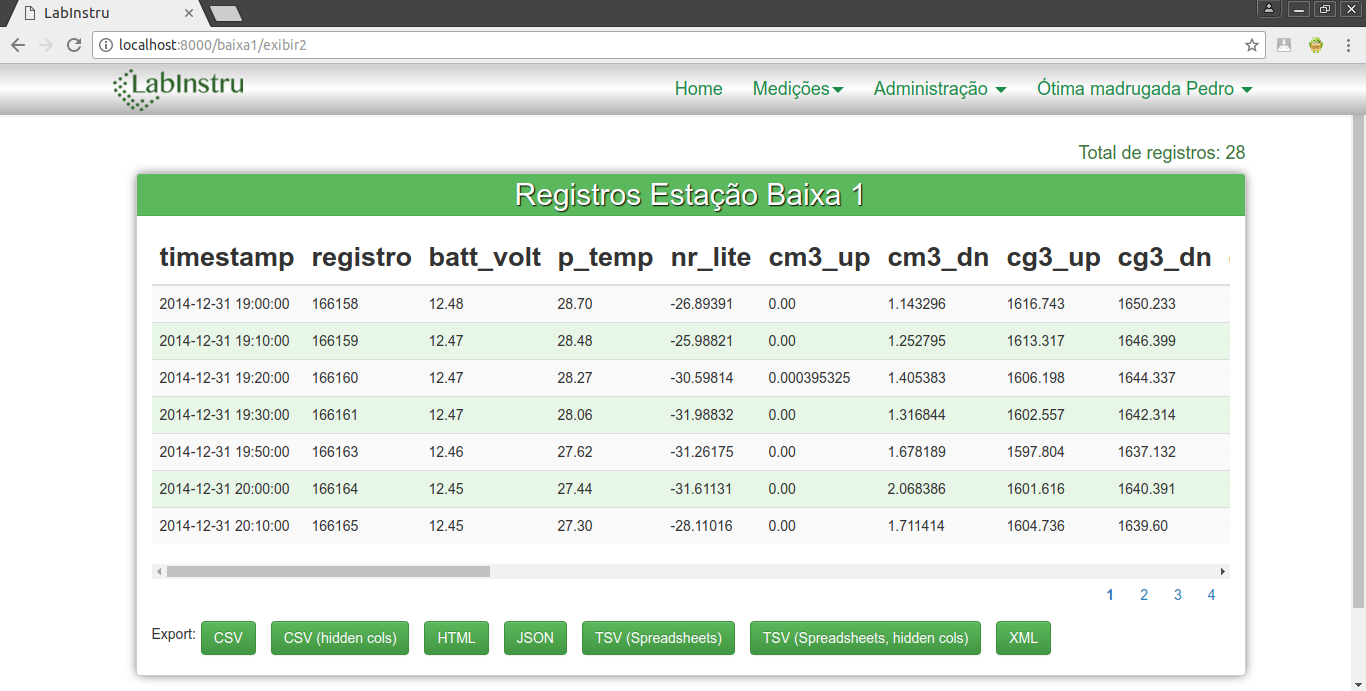
\includegraphics[width=0.7\linewidth]{./img/ap7}}
\caption{Resultado da consulta de medições.}
\end{figure}
\end{frame}

\begin{frame}{Solução Proposta: Funcionalidades Implementadas}
\begin{figure}[h!]
\centering
\frame{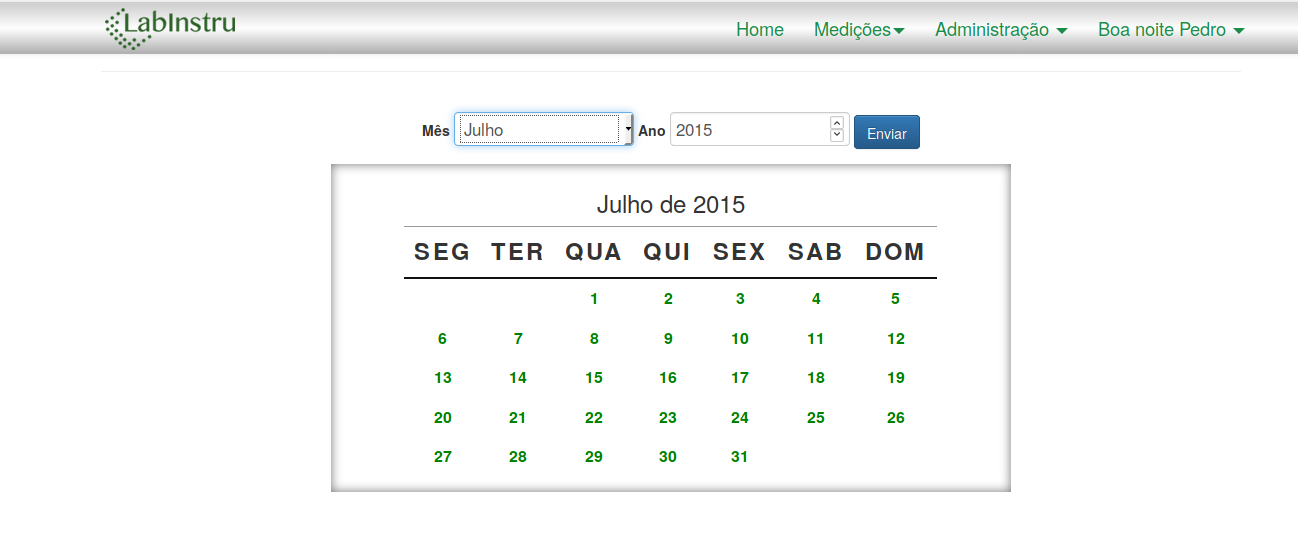
\includegraphics[width=0.7\linewidth]{./img/disponibilidade2}}
\caption{Verificação de disponibilidade}
\end{figure}
\end{frame}

\begin{frame}{Apresentação LabInstru Web}
	\begin{center}
	\movie[width=160px, height=90px, externalviewer]{Vídeo de ilustração de algumas funcionalidades.}{video/video.mp4}
	\end{center}
\end{frame}

\begin{frame}{Boletim Meteorológico Diário}
\begin{itemize}
	\item Uma das atividades promovidas pelo LabInstru
	\item Importante informativo sobre clima e tempo de nossa região
  \item Divulgação das informações junto à comunidade
	\item Possui várias informações derivadas dos dados obtidos da estação meteorológica
	\begin{itemize}
		\item Índice de Calor
		\item Escala de Beaufort
	\end{itemize}
	\item Elaboração de modelo para o boletim meteorlógico
	\item Implementação a partir do modelo
\end{itemize}
\end{frame}

\begin{frame}{Modelo para Boletim Meteorológico Diário}
\begin{figure}[h!]
\centering
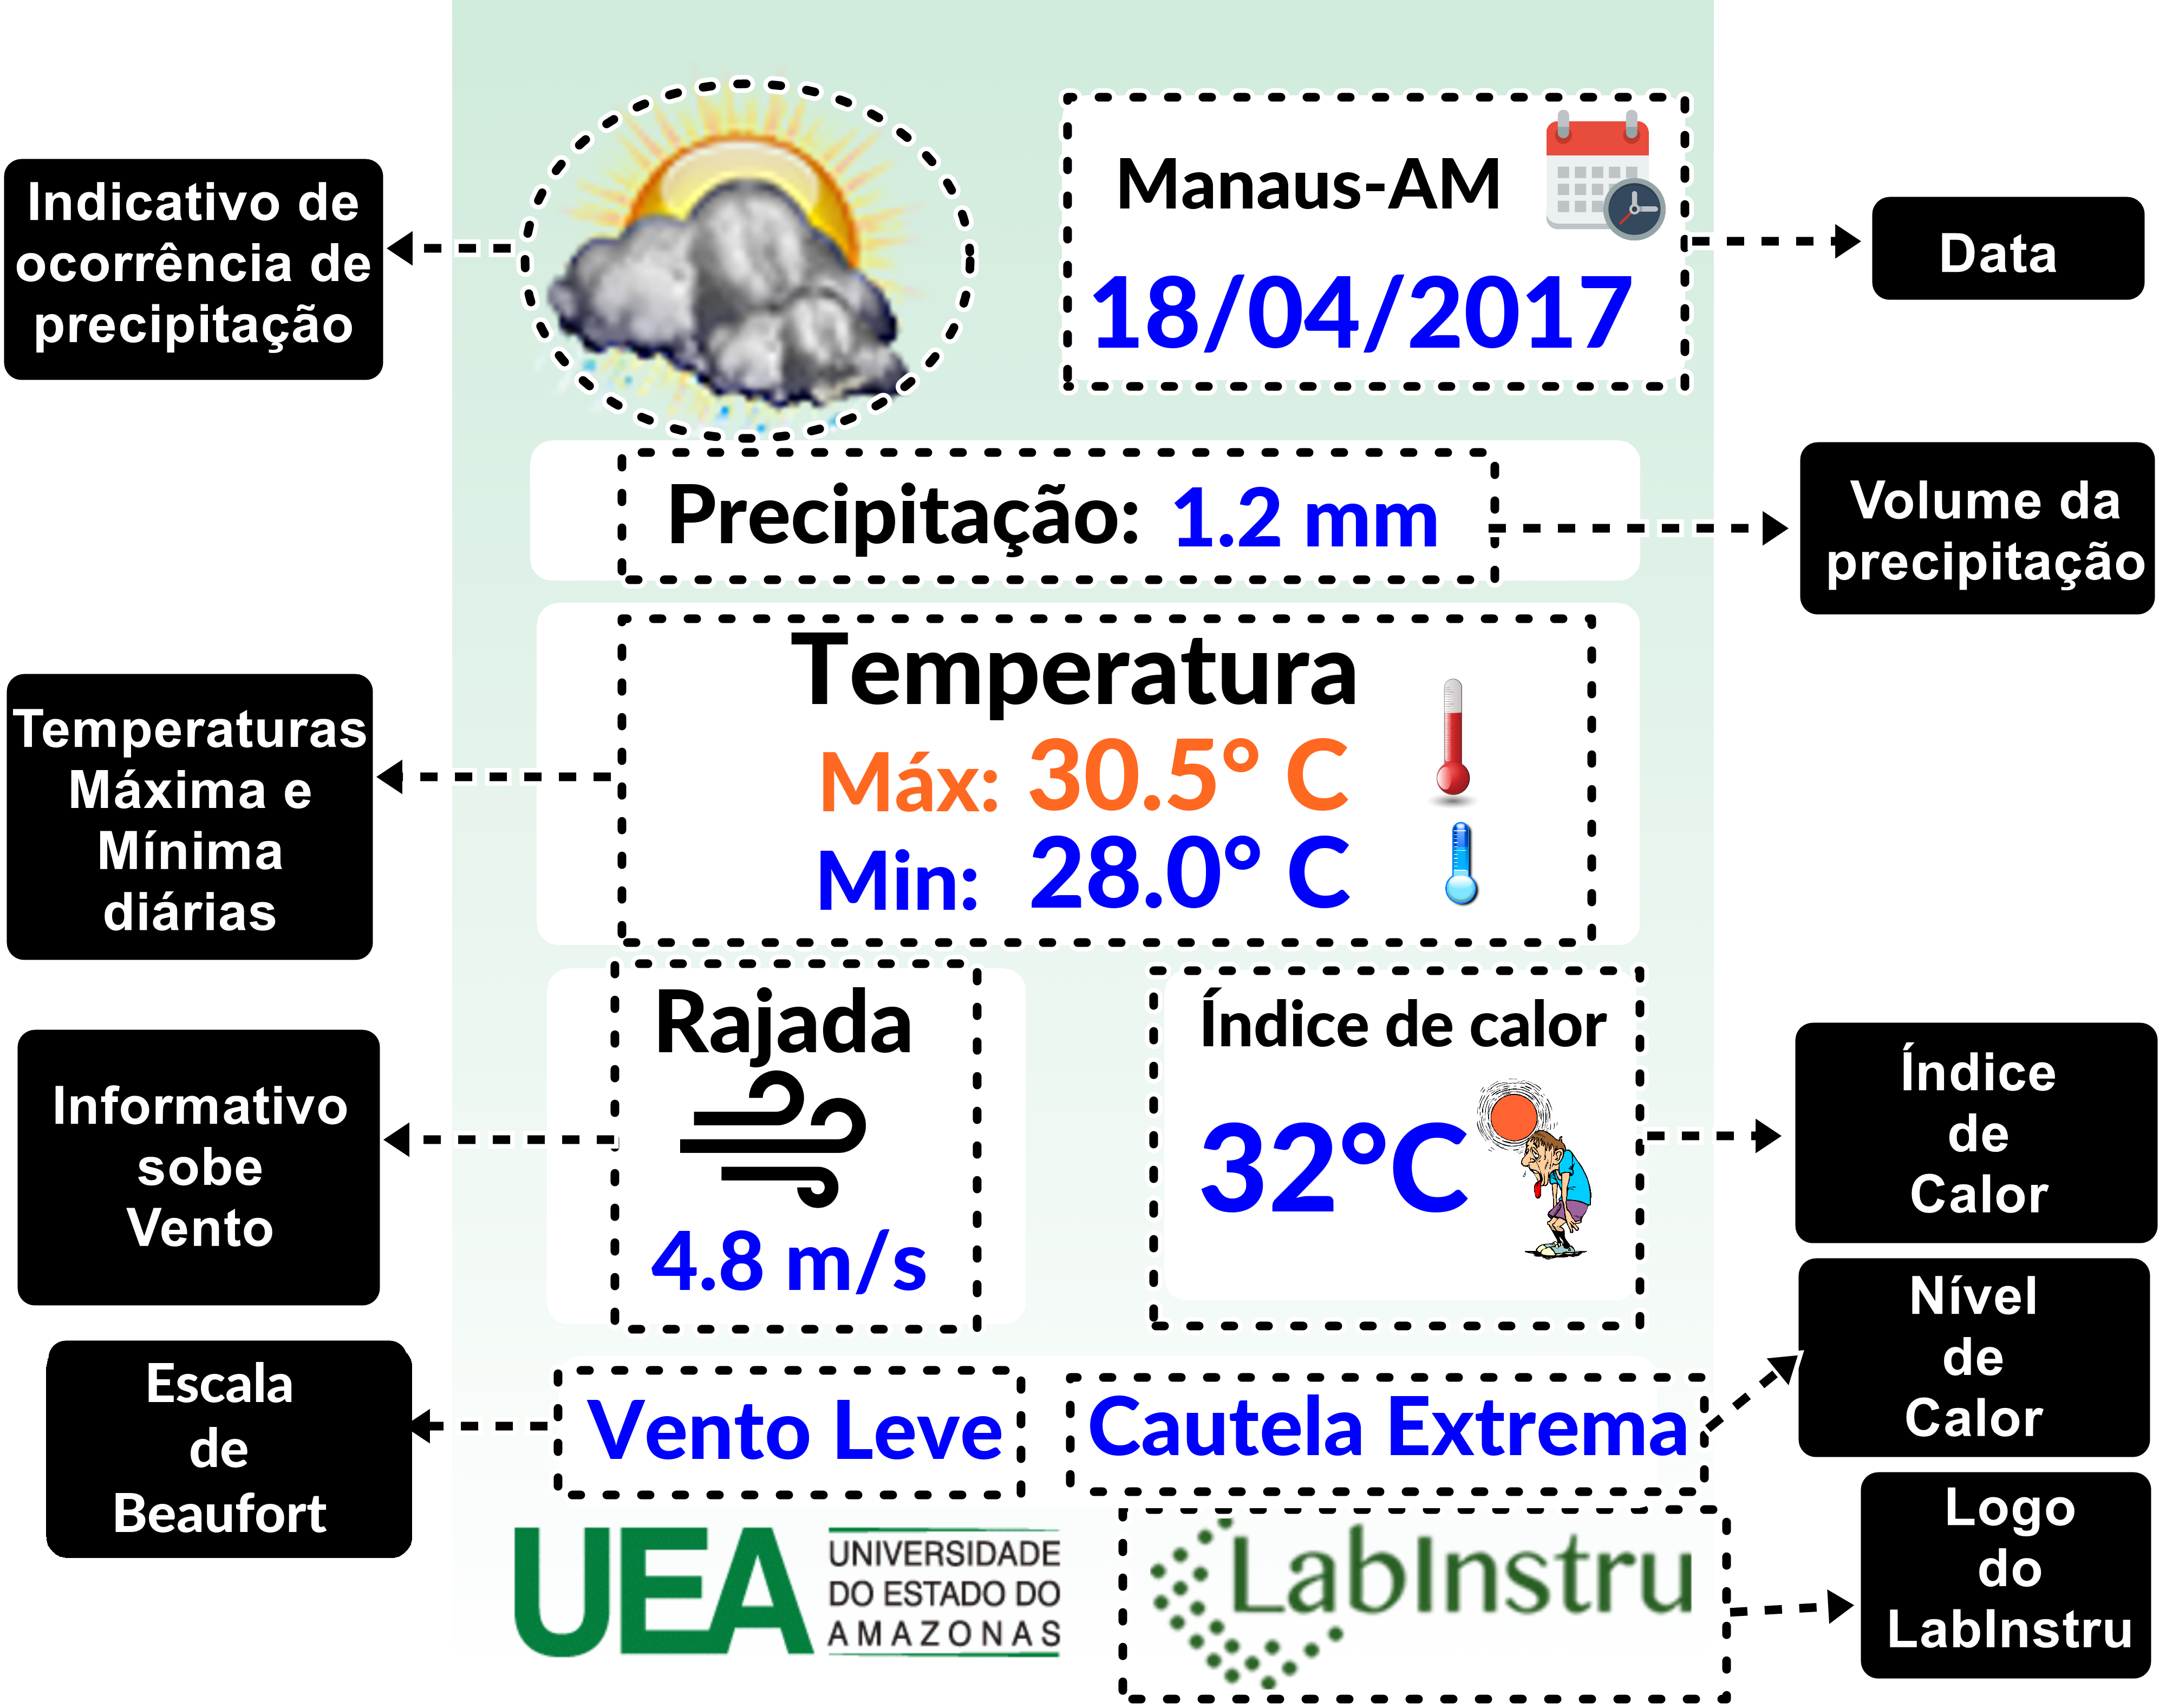
\includegraphics[width=0.5\linewidth]{./img/esbocoBoletim}
\caption{Modelo elaborado para o boletim meteorológico} \label{fig:modeloBoletim}
\end{figure}
\end{frame}

\begin{frame}{Boletim Meteorológico Diário Implementado}
\begin{figure}[h!]
\centering
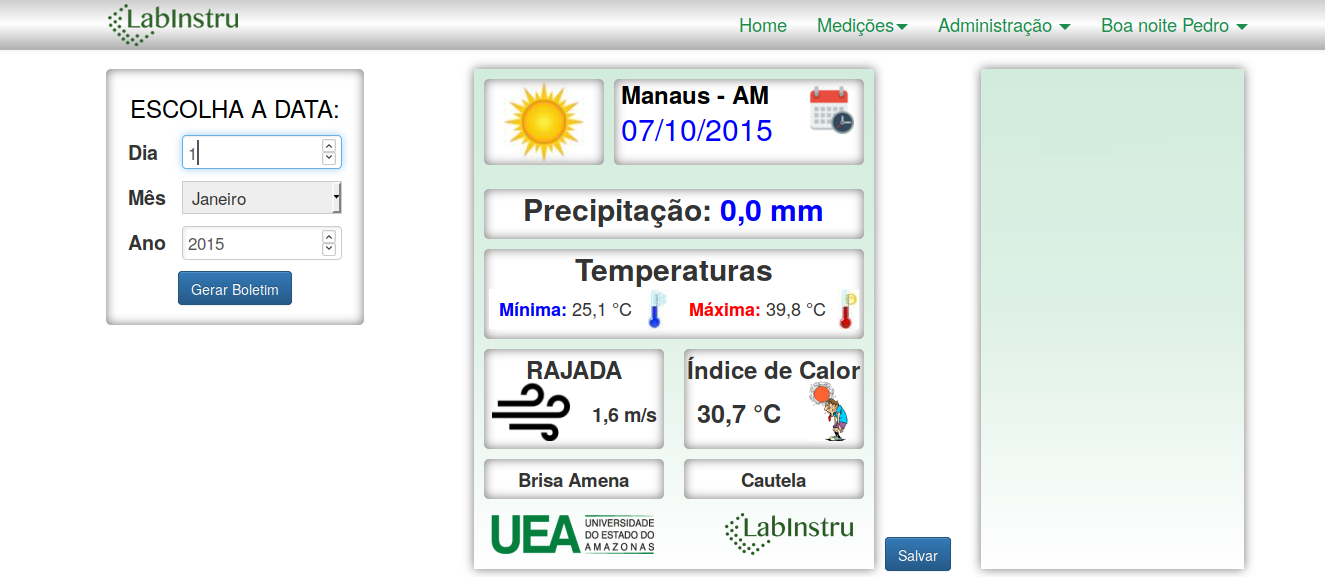
\includegraphics[width=0.7\linewidth]{./img/boletim}
\caption{Boletim meteorológico implementado no LabInstru Web} \label{fig:boletim}
\end{figure}
\end{frame}

\begin{frame}{Métricas de Software}
\begin{itemize}
\item Linhas de código: 7264 no total, sendo:
\begin{itemize}
\item[-] Arquivos Python: 1714 linhas
\item[-] Arquivos HTML: 2400 linhas
\item[-] Arquivos de estilo: 3150 linhas
\end{itemize}
\ \ \newline
\item Funções disponíveis no Controller: 28
\begin{itemize}
	\item Analogia com web services
\end{itemize}
\ \ \newline
\item Modelo de dados: 8
\begin{itemize}
	\item Acordância com a modelagem efetuada anteriormente
\end{itemize}
\end{itemize}
\end{frame}


\begin{frame}{Implantação da Solução Proposta}
\begin{itemize}
	\item Realizada com o \alert{Google App Engine}
	\begin{itemize}
		\item Plataforma em nuvem
		\item Total suporte à linguagem Python
		\item Nível de serviço gratuito
		\item Alta disponibilidade e baixa latência
	\end{itemize}
	\ \ \newline
	\item \alert{Status atual}: Corrigindo detalhes de implantação para disponibilização aos pesquisadores e estudantes do LabInstru
\end{itemize}
\end{frame}


\section{Considerações Finais}
\begin{frame}{Considerações Finais}
\begin{itemize}
\item LabInstru Web: projeto e implementação de uma \alert{plataforma web} para o LabInstru
\ \ \newline
\item Prover armazenamento, gerenciamento e disponibilização dos dados de forma automática
\ \ \newline
\item Geração automática dos boletins meteorológicos
\ \ \newline
\item Escolha de metodologias e ferramentas ágeis para o desenvolvimento da aplicação
\end{itemize}
\end{frame}

\begin{frame}{Considerações Finais}
\begin{itemize}
\item Identificação de novas funcionalidades a serem desenvolvidas
\ \ \newline
\item Refinar requisitos já implementados
\ \ \newline
\item Avaliar a performance da solução implantada
\ \ \newline
\item Integração do LabInstru Web com aprendizado de máquina (\alert{machine learning})
\end{itemize}
\end{frame}

\maketitle


\end{document}
